\documentclass{article}
\usepackage{tikz}

\begin{document}

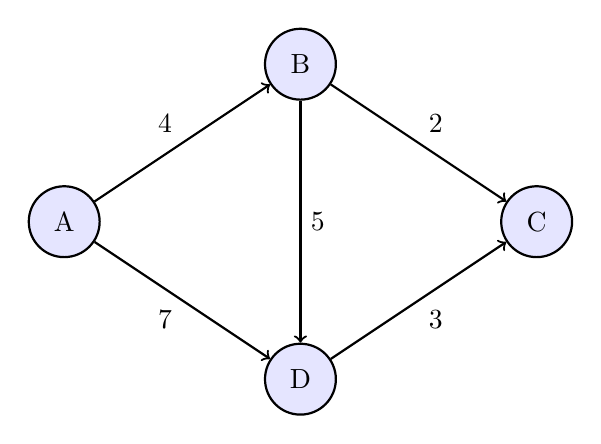
\begin{tikzpicture}[
    vertex/.style={
        circle,
        draw,
        thick,
        minimum size=9mm,
        fill=blue!10
    },
    edge/.style={
        ->,
        thick
    }
]

    \node[vertex] (A) at (0,2) {A};
    \node[vertex] (B) at (3,4) {B};
    \node[vertex] (C) at (6,2) {C};
    \node[vertex] (D) at (3,0) {D};

    \draw[edge] (A) -- node[above left] {4} (B);
    \draw[edge] (B) -- node[above right] {2} (C);
    \draw[edge] (A) -- node[below left] {7} (D);
    \draw[edge] (D) -- node[below right] {3} (C);
    \draw[edge] (B) -- node[right] {5} (D);

\end{tikzpicture}

\end{document}
